%\chapter{Cybersecurity Education}\label{ch:discussion}
%In this chapter, the importance of cybersecurity education is highlighted, and the potential use cases for the RCSL in education are layed out.
%
%\section{Importance of Cybersecurity Education}
%The advancement of digital information technology, accelerated by trends like Artificial Intelligence, Cloud Computing or the Internet of Things (IoT), has reached a high pace, which companies and institutions are trying to keep up with.
%In the pursuit of keeping up with this pace, convenience is often the main focus, whereas security and privacy are left as an afterthought. \cite[chapter~1]{Salmon_Levesque_McLafferty_2017}
%This leads to the implementation and operation of vulnerable systems, presenting a larger attack surface for cybercriminals.
%
%Experts estimate that cybercrime causes annual damages of 110 billion dollars worldwide and most companies, relying heavily on their IT infrastructure, can only operate for a few days without these systems \cite[page~3]{Hellmann_2023},\cite[page~12]{Salmon_Levesque_McLafferty_2017}. 
%cyberattacks in the form of data piracy, or blackmailing have become commonplace and cause ever-increasing financial damages for companies, the public, and governments, as seen in the example depicted in \cref{fig:cost_of_cybercrime}.
%
%\begin{figure}[h]
%    \centering
%    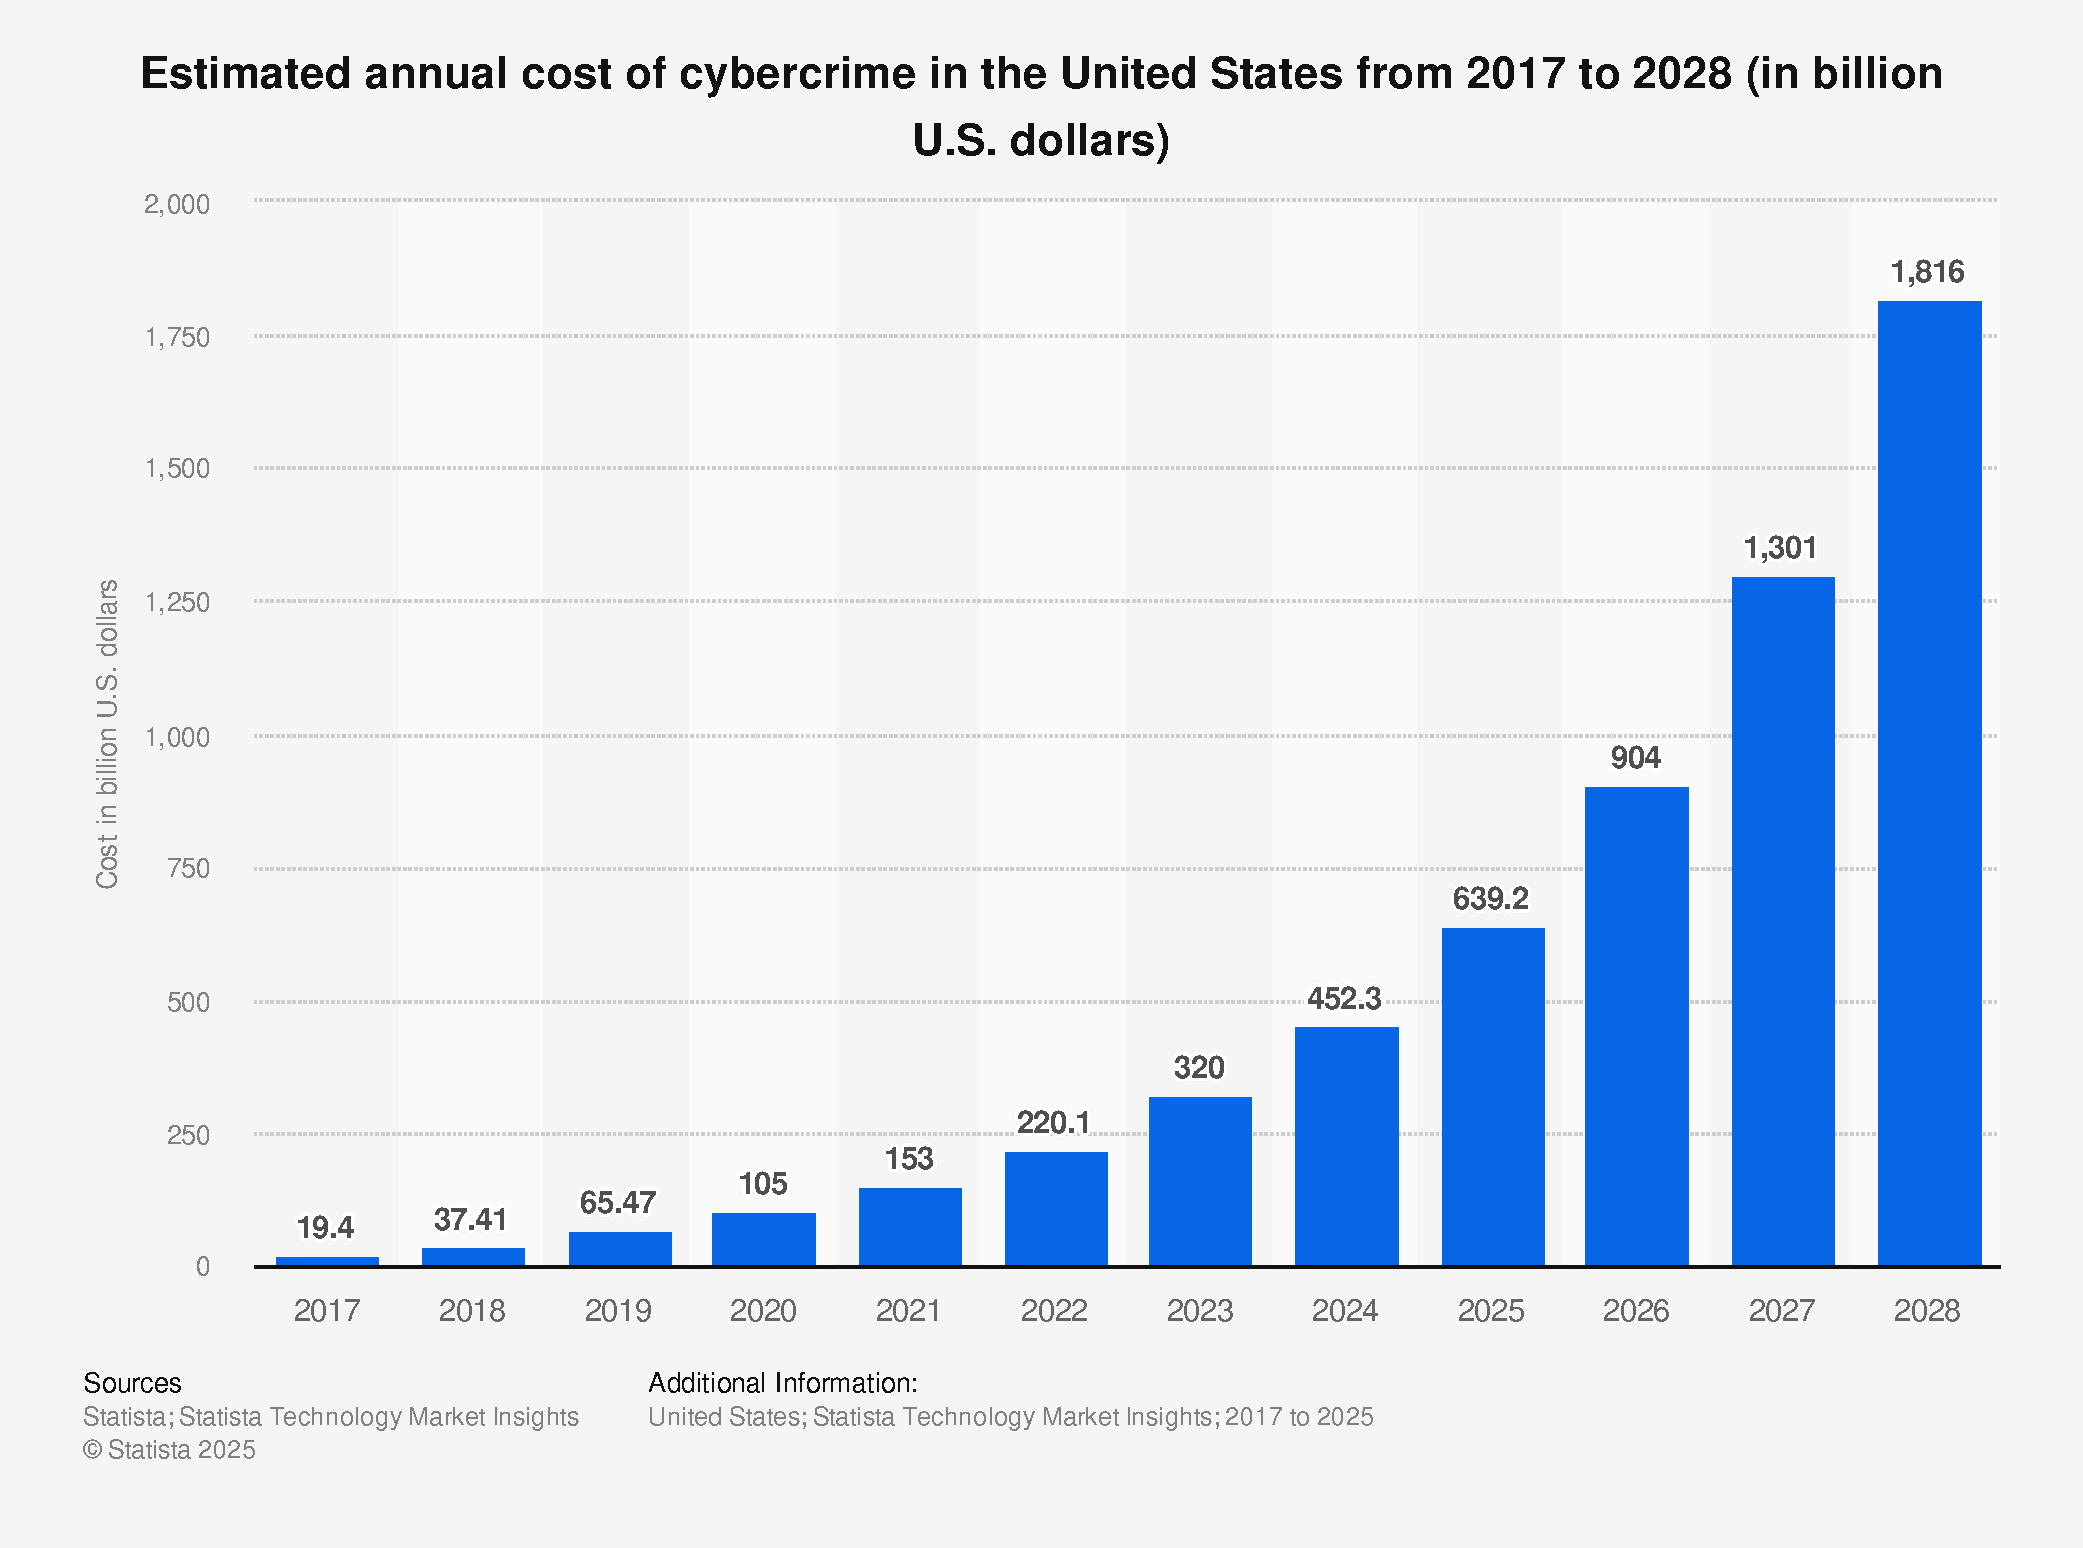
\includegraphics[width=0.8\textwidth]{figures/Abbildungen/statistic_id1399040_annual-cost-of-cybercrime-in-the-us-2017-2028.pdf}
%    \caption{Estimated annual cost of cybercrime in the United States from 2017 to 2028 \cite{statista_cc}}
%    \label{fig:cost_of_cybercrime}
%\end{figure}
%
%Cybersecurity awareness and education play a large role in ensuring the integrity of networks and systems. 
%People without awareness and training in cybersecurity oftentimes tend to circumvent or ignore security mechanisms since following the principles of cybersecurity is often connected to effort \cite{Hellmann_2023}.
%Awareness training should educate about the potential threads in the cyberspace and security measures to apply for mitigating the risk of falling victim to cybercrime.
%Futhermore, the training should sensitize for common schemes of Social Engineering.
%This helps to protect against threads like Social Engineering, Malware, or network attacks, such as MitM or Evil Twin. \cite[page~24-25]{IT_Basiswissen}, \cite{mariano2024wifi}
%
%\section{Results Evaluation}
%The general usability of the RCSL proved to be in line with the goals set for the project with intuitive and smooth operation.
%The software architecture is mostly modular, allowing future expansion, and executes correctly implemented functions reliably.
%For improved development and problem analysis as well as performance, a rewrite of the code with adherence to software engineering best practices would be adviceable.
%
%Concluding the tests, it appears the RCSL can provide a relatively reliable environment to perform network attacks in.
%However, the generation of artificial network traffic could aid the speed of cracking WEP, as well as depict a more realistic scenario, and might be considered for future improvements.
%The error caused by wpa\_supplicant, described in \cref{sec:network_management}, seems to have been fixed, but should also be revisited in order to implement a more dependable fix.
%
%
%\section{Potential Use Cases}
%Confrontation with realistic scenarios and hands-on practice are effective tools for raising awareness and teaching cybersecurity.
%Authentic experiences help to "reinforc[e] the importance of [security]" \cite{mariano2024wifi} and connect previously learned theory to the experience in real world application. 
%Providing context for learning is essential, as it helps to build mental schemas and understanding of the core concepts, enhancing the ability to transfer the knowledge to different scenarios. \cite[page~61]{Cybersec_Edu}
%
%The RCSL is able to create test environments for various applications and could be used as tool in education for demonstration purposes and to allow students to get hands-on experience.
%
%A lecturer could use the device to demonstrate the process of cracking a Wi-Fi network and performing subsequent attacks like MitM to eavesdrop on the traffic.
%The MQTT communication between the RPI and ESP32 could be a suitable target for such an attack.
%Demonstration of the ease with which an improperly secured network can be cracked and data stolen or manipulated would most likely give a vivid impression of the threats present in the cyberspace.
%This memorable experience intern might lead to the perception of the importance of cybersecurity being increased, aiding the spread of awareness.
%
%For cybersecurity students, the RCSL could serve as a platform to practice pentesting techniques on, providing context for theoretical concepts and practical experience.
%The attacks performed in \cref{ch:testing} are an obvious choice as well as various network attacks, such as MitM, DoS, or TLS/SSL attacks.
%Besides pentesting, future expansions of the project could also include the implementation of protective measures, such as IDS systems, allowing students to gain experience in their application.
%
%The Juice Shop could be employed for teaching security practices in software engineering and web development, providing context for the adherence to principles of secure development.
%
%With the future addition of features, like the ones suggested in \cref{ch:outlook}, the RCSL could be expanded to cater for numerous further use cases.